\part{Introduction}

\section{Introduction}

\subsection{About this course}

\begin{frame}{Hello World}{}
  \begin{center}
    \sourceinput{snippets/hello.cc}
  \end{center}
\end{frame}

\begin{frame}{Objective}{}
  \begin{block}{Objective}
    Learn how to use different paradigms in a single application with modern \CCLang

    \begin{itemize}
    \item
      procedural programming
    \item
      object-oriented programming
    \item
      functional programming
    \item
      generic programming
    \end{itemize}
  \end{block}
\end{frame}

\begin{frame}{Organisation}{}
  \begin{block}{Hours}
    \begin{itemize}
    \item
      Lecture: 5 $\times$ 1h30
    \item
      Test: 1 $\times$ 1h30
    \item
      Laboratory: 6 $\times$ 3h00
    \end{itemize}
  \end{block}

  \begin{block}{Evaluation}
    \begin{itemize}
    \item
      Multiple choice test (50\%)
    \item
      Laboratory project in \CCLang (50\%)
    \end{itemize}
  \end{block}
\end{frame}

\begin{frame}{Resources}{}
  \begin{block}{Online}
    \begin{itemize}
    \item
      \CCLang Reference: \url{http://en.cppreference.com/w/cpp}
    \item
      \CCLang FAQ: \url{http://isocpp.org/faq}
    \item
      \CCLang Core Guidelines: \url{https://github.com/isocpp/CppCoreGuidelines/}
    \end{itemize}
  \end{block}

  \begin{block}{Books}
    \begin{thebibliography}{}
    \bibitem{Stroustrup}
      Bjarne Stroustrup.
      \newblock {\em The \CCLang Programming Language}.
      \newblock 4th edition, 2013, Addison--Wesley
    \end{thebibliography}
  \end{block}
\end{frame}

\subsection{\CCLang Origins}

% Source: "Evolving a language in and for the real world: 1991-2006", Bjarne Stroustrup

\begin{frame}{\CCLang History (1/3)}{Early \CCLang}
  \begin{block}{Early \CCLang (1979--1998)}
    \begin{itemize}
    \item
      1979: "C with Classes", Bjarne Stroustrup, AT\&T Bell Labs
    \item
      1983: "C with Classes" $\leadsto$ \CCLang; CFront 1.0
    \item
      1985: \emph{The \CCLang Programming Language}, 1st edition, Bjarne Stroustrup
    \item
      1989: \emph{The Annotated \CCLang Reference Manual}, Bjarne Stroustrup; CFront 2.0
    \item
      1991: First ISO/IEC JTC1/SC22/WG21 meeting; CFront 3.0
    \item
      1992: \emph{Effective \CCLang}, 1st edition, Scott Meyers
    \item
      1993: Standard Template Library, Alexander Stepanov, HP Labs
    \item
      1994: \emph{The Design and Evolution of \CCLang}, Bjarne Stroustrup
    \item
      1998: \emph{Effective \CCLang}, 2nd edition, Scott Meyers
    \end{itemize}
  \end{block}
\end{frame}

\begin{frame}{\CCLang History (2/3)}{Standard \CCLang}
  \begin{block}{Standard \CCLang (1998--2011)}
    \begin{itemize}
    \item
      1998: ISO standardization, \CC{98}
    \item
      2001: \emph{Modern \CCLang Design}, Andrei Alexandrescu
    \item
      2003: \CC{03}, minor revision
    \item
      2005: \emph{Effective \CCLang}, 3rd edition, Scott Meyers
    \item
      2006: Performance Technical Report
    \item
      2007: Library Technical Report 1 (TR1)
    \end{itemize}
  \end{block}
\end{frame}

\begin{frame}{\CCLang History (3/3)}{Modern \CCLang}
  \begin{block}{Modern \CCLang (2011--)}
    \begin{itemize}
    \item
      2011: \CC{11}, major revision
      \begin{itemize}
      \item[$\to$]
        "Surprisingly, \CC{11} feels like a new language"
      \end{itemize}
    \item
      2012: Standard \CCLang Foundation
    \item
      2014: \CC{14}, minor revision; \emph{Effective Modern \CCLang}, Scott Meyers
    \item
      2015: \CCLang Core Guidelines, Guidelines Support Library
    \item
      2017: \CC{17}, major revision
    \item
      2020: \CC{20}, next major revision of the standard
    \end{itemize}
  \end{block}
\end{frame}

\begin{frame}{Design Rules (1/4)}{General rules}
  \begin{block}{General rules}
    \begin{enumerate}
    \item
      \CCLang's evolution must be driven by real problems.
    \item
      Don't get involved in a sterile quest for perfection.
    \item
      \CCLang must be useful \emph{now}.
    \item
      Every feature must have a reasonably obvious implementation.
    \item
      Always provide a transition path.
    \item
      \CCLang is a language, not a complete system.
    \item
      Provide comprehensive support for each supported style.
    \item
      Don't try to force people to use a specific programming style.
    \end{enumerate}
  \end{block}
\end{frame}

\begin{frame}{Design Rules (2/4)}{Design support rules}
  \begin{block}{Design support rules}
    \begin{enumerate}
    \item
      Support sound design notions.
    \item
      Provide facilities for program organization.
    \item
      Say what you mean.
    \item
      All features must be affordable.
    \item
      It is more important to allow a useful feature than to prevent every misuse.
    \item
      Support composition of software from separately developed parts.
    \end{enumerate}
  \end{block}
\end{frame}

\begin{frame}{Design Rules (3/4)}{Language-technical rules}
  \begin{block}{Language-technical rules}
    \begin{enumerate}
    \item
      No implicit violations of the static type system.
    \item
      Provide as good support for user-defined types as for built-in types.
    \item
      Locality is good.
    \item
      Avoid order dependencies.
    \item
      If in doubt, pick the variant of a feature that is easiest to teach.
    \item
      Syntax matters (often in perverse ways).
    \item
      Preprocessor usage should be eliminated.
    \end{enumerate}
  \end{block}
\end{frame}

\begin{frame}{Design Rules (4/4)}{Low-level programming support rules}
  \begin{block}{Low-level programming support rules}
    \begin{enumerate}
    \item
      Use traditional (dumb) linkers.
    \item
      No gratuitous incompatibilities with C.
    \item
      Leave no room for a lower-level language below C++ (except assembler).
    \item
      What you don’t use, you don’t pay for (zero-overhead rule).
    \item
      If in doubt, provide means for manual control.
    \end{enumerate}
  \end{block}
\end{frame}

\subsection{\CCLang Paradigms}

\begin{frame}{Programming paradigm}{}
  \begin{definition}[Programming paradigm]
    A \strong{programming paradigm} is a way to think about the execution and/or the organization of a program. A programming paradigm enables some constructs in a language and forbids other constructs.
  \end{definition}

  \begin{block}{Remarks}
    \begin{itemize}
    \item
      There are dozens of programming paradigms.
    \item
      Most languages can be classified into multiple paradigms (like \CCLang).
    \end{itemize}
  \end{block}

  \begin{example}[Imperative programming]
    \strong{Imperative programming} is a paradigm that uses a sequence of statements to change the program's state.
  \end{example}
\end{frame}

\begin{frame}{Procedural programming}{}
  \begin{definition}[Procedural programming]
    \strong{Procedural programming} is an imperative programming paradigm based on the concept of \emph{procedure call}.
  \end{definition}
  \begin{block}{Procedural programming in \CCLang}
    \CCLang is a procedural programming language.
    \begin{itemize}
    \item
      Modularity through function parameters and return values
    \item
      Function call from any other function
    \item[$\to$]
      C style
    \end{itemize}
  \end{block}
\end{frame}

\begin{frame}{Object-oriented programming}{}
  \begin{definition}[Object-oriented programming]
    \strong{Object-oriented programming} is an imperative programming paradigm based based on the concepts of \emph{objects} (data) and \emph{methods} (code).
  \end{definition}
  \begin{block}{Object-oriented programming in \CCLang}
    \CCLang is an object-oriented programming language.
    \begin{itemize}
    \item
      Classes (\lstinline!class!)
      \begin{itemize}
      \item[$\to$]
        Class-based object-oriented programming ($\neq$ Prototype-based)
      \end{itemize}
    \item
      Composition and (multiple) inheritance
    \item
      Polymorphism (\lstinline!virtual! methods, \lstinline!dynamic_cast!)
    \end{itemize}
  \end{block}
\end{frame}

\begin{frame}{Functional programming}{}
  \begin{definition}[Functional programming]
    \strong{Functional programming} is a programming paradigm based on the concept of \emph{mathematical functions} and forbids side effects (no assignment).
  \end{definition}
  \begin{block}{Functional programming in \CCLang}
    \CCLang is \strong{not} a functional programming language\ldots
    \begin{itemize}
    \item
      No currying
    \end{itemize}
    \ldots but has elements of a functional programming language.
    \begin{itemize}
    \item
      Recursion
    \item
      Functors and lambda functions\Since{11} (closures)
    \item
      \lstinline!std::function!\Since{11}
    \item
      Partial evaluation (\lstinline!std::bind!)
    \end{itemize}
  \end{block}
\end{frame}

\begin{frame}{Generic programming}{}
  \begin{definition}[Generic programming]
    \strong{Generic programming} is a programming paradigm where types and algorithms are defined with abstract type parameters.
  \end{definition}
  \begin{block}{Generic programming in \CCLang}
    \CCLang is a generic programming language.
    \begin{itemize}
    \item
      Templates
    \item
      Standard Template Library (STL): containers, iterators, algorithms
    \item
      Concepts\Since{20}
    \end{itemize}
  \end{block}
\end{frame}

\begin{frame}{Using multiple paradigms}{}
  \begin{example}
    \sourceinput{snippets/multi_paradigm.cc}

    \begin{itemize}
    \item
      Procedural: \lstinline!drawAll()!
    \item
      Object-oriented: \lstinline!shape->draw()!
    \item
      Functional: \lstinline![](const Shape *shape) \{ \}!
    \item
      Generic: \lstinline!std::vector<Shape*>! and \lstinline!std::for_each!
    \end{itemize}
  \end{example}
\end{frame}


\section{Expressions and declaration in \CCLang}

\subsection{Overview}

\begin{frame}{\CCLang program}{}
  \begin{definition}[\CCLang program]
    A \strong{\CCLang program} is a sequence of text files (typically header and source files) that contain declarations. They undergo translation to become an executable program, which is executed when the C++ implementation calls its main function.
  \end{definition}
\end{frame}

\begin{frame}{Entities}{}
  \begin{block}{Entities}
    The \strong{entities} of a C++ program are:
    \begin{itemize}
    \item
      values
    \item
      objects
    \item
      references
    \item
      structured bindings\Since{17}
    \item
      functions
    \item
      enumerators
    \item
      types
    \item
      class members
    \item
      templates
    \item
      template specializations
    \item
      namespaces
    \item
      parameter packs.
    \end{itemize}
  \end{block}
\end{frame}

\begin{frame}{Objects}{}
  \begin{definition}[Object]
    An \strong{object} is a \emph{region of storage} with the following properties:
    \begin{itemize}
    \item
      a size (that can be determined with \lstinline!sizeof!)
    \item
      an alignment requirement (that can be determined with \lstinline!alignof!)
    \item
      a storage duration (automatic, static, dynamic, thread-local)
    \item
      a lifetime
    \item
      a type
    \item
      a value (which may be indeterminate)
    \item
      optionally, a name
    \end{itemize}
  \end{definition}
\end{frame}


\subsection{Value categories}

\begin{frame}{Expressions}{}
  \begin{block}{Expressions}
    Expressions are characterized by two properties:
    \begin{itemize}
    \item
      a \emph{type}
    \item
      a \emph{value category}
    \end{itemize}
  \end{block}

  \begin{block}{Value categories before \CC{11}}
    \begin{itemize}
    \item
      An \strong{lvalue expression} identifies an object ("locator value")
      \begin{itemize}
      \item[$\approx$]
        what is on the left-hand side  of an assignment
      \end{itemize}
    \item
      A \strong{rvalue expression} is an expression that is not an lvalue expression
      \begin{itemize}
      \item[$\approx$]
        what is on the right-hand side of an assignment
      \end{itemize}
    \end{itemize}
  \end{block}
\end{frame}

\begin{frame}{Value categories}{Overview}
  \begin{block}{Value categories}
    \begin{itemize}
    \item
      Primary categories: lvalue, prvalue, xvalue
    \item
      Mixed categories: glvalue, rvalue
    \end{itemize}
  \end{block}

  \begin{center}
    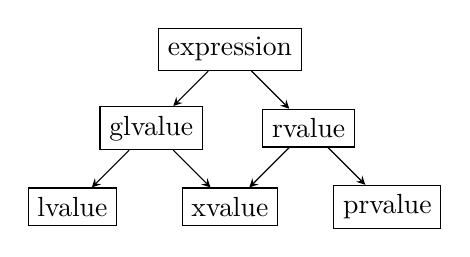
\begin{tikzpicture}
      \node[draw] (E) at ( 0, 0) { expression } ;
      \node[draw] (G) at (-1,-1) { glvalue } ;
      \node[draw] (R) at ( 1,-1) { rvalue } ;
      \node[draw] (L) at (-2,-2) { lvalue } ;
      \node[draw] (X) at ( 0,-2) { xvalue } ;
      \node[draw] (P) at ( 2,-2) { prvalue } ;

      \draw[->,>=stealth] (E) -- (G) ;
      \draw[->,>=stealth] (E) -- (R) ;
      \draw[->,>=stealth] (G) -- (L) ;
      \draw[->,>=stealth] (G) -- (X) ;
      \draw[->,>=stealth] (R) -- (X) ;
      \draw[->,>=stealth] (R) -- (P) ;
    \end{tikzpicture}
  \end{center}
\end{frame}

% http://www.open-std.org/jtc1/sc22/wg21/docs/papers/2015/p0135r0.html
\begin{frame}{Value categories}{Definition (\CC{17})}
  \begin{definitions}[Value categories]
    \begin{itemize}
    \item
      A \strong{glvalue} ("generalized" lvalue) is an expression whose evaluation determines the identity of an object, bit-field, or function
      \begin{itemize}
      \item[$\to$]
        \emph{glvalues produce locations}
      \end{itemize}
    \item
      A \strong{prvalue} ("pure" rvalue) is an expression whose evaluation either:
      \begin{itemize}
      \item
        computes the value of the operand of an operator (has no result object), or
      \item
        initializes an object or a bit-field (has a result object)
      \item[$\to$]
        \emph{prvalues perform initialization}
      \end{itemize}
    \item
      An \strong{xvalue} (eXpiring value) is a glvalue that denotes an object or bit-field whose resources can be reused (usually near the end of its lifetime)
    \item
      An \strong{lvalue} is a glvalue that is not an xvalue
    \item
      An \strong{rvalue} is a prvalue or an xvalue.
    \end{itemize}
  \end{definitions}
\end{frame}

\begin{frame}{Properties of glvalues and rvalues}{}
  \begin{block}{Properties of a glvalue expression (lvalue or xvalue)}
    \begin{itemize}
    \item
      May be converted to a prvalue
    \item
      May be polymorphic (dynamic type $\neq$ static type)
    \item
      Can have incomplete type
    \end{itemize}
  \end{block}

  \begin{block}{Properties of a rvalue expression (prvalue or xvalue)}
    \begin{itemize}
    \item
      Has no address
    \item
      Can not be used as the left-hand of the built-in assignment operator
    \item
      May be used to initialize a const lvalue reference or an rvalue reference
      \begin{itemize}
      \item[$\to$]
        In that case, the lifetime of the object identified by the rvalue is extended until the scope of the reference ends
      \end{itemize}
    \end{itemize}
  \end{block}
\end{frame}

\begin{frame}{Properties of lvalues and prvalues}{}
  \begin{block}{Properties of an lvalue expression}
    \begin{itemize}
    \item
      Has an address
    \item
      If modifiable, may be used as the left-hand of the built-in assignment operator
    \item
      May be used to initialize an lvalue reference
    \end{itemize}
  \end{block}

  \begin{block}{Properties of an prvalue expression}
    \begin{itemize}
    \item
      Can not be polymorphic
    \item
      If non-class and non-array, can not cv-qualified
    \item
      Can not have incomplete type
    \item
      Can not have abstract class type
    \end{itemize}
  \end{block}
\end{frame}

\begin{frame}{Examples of lvalues}{}
  \begin{examples}[lvalue expressions]
    \begin{itemize}
    \item
      Name of a variable, function, data member (\lstinline!std::cin!)
    \item
      Function call or overloaded operator expression whose return type is lvalue reference (\lstinline!std::getline(std::cin, str)!, \lstinline!std::cout << 1!, \lstinline!++it!)
    \item
      Assignment and compound assignment expressions (\lstinline!a = b!, \lstinline!a += b!)
    \item
      Builtin pre-increment and pre-decrement expressions (\lstinline!++i!)
    \item
      Builtin indirection expression (\lstinline!*p!)
    \item
      Builtin subscript operator\manualfootnote (\lstinline!a[n]!)
    \item
      String literal (\lstinline!"Hello"!)
    \item
      Member of object expressions\manualfootnote (\lstinline!a.m!)
    \item
      Built-in member of pointer expression\manualfootnote (\lstinline!a->m!)
    \end{itemize}

    \raggedleft
    \footnotesize
    \manualfootnote with exceptions
  \end{examples}
\end{frame}

\begin{frame}{Examples of prvalues}{}
  \begin{examples}[prvalue expressions]
    \begin{itemize}
    \item
      Literal\manualfootnote (\lstinline!42!, \lstinline!true!, \lstinline!nullptr!)
    \item
      Function call or an overloaded operator expression whose return type is non-reference (\lstinline!str.substr(1, 2)!, \lstinline!it++!)
    \item
      Builtin post-increment and post-decrement expressions (\lstinline!i++!)
    \item
      Builtin arithmetic expressions (\lstinline!a + b!, \lstinline!a / b!, \lstinline!a & b!, \lstinline!a << b!, \lstinline!-a!)
    \item
      Builtin logical expressions (\lstinline!a && b!, \lstinline!a || b!, \lstinline|!a|)
    \item
      Builtin comparison expressions (\lstinline!a < b!, \lstinline!a == b!)
    \item
      Builtin address-of expression (\lstinline!&a!)
    \item
      The \lstinline!this! pointer
    \item
      Enumerator
    \item
      Lambda expression (\lstinline![](int x){ return x * x; }!)
    \end{itemize}

    \raggedleft
    \footnotesize
    \manualfootnote with exceptions
  \end{examples}
\end{frame}

\begin{frame}{Examples of xvalues}{}
  \begin{examples}[xvalue expressions]
    \begin{itemize}
    \item
      Function call or an overloaded operator expression, whose return type is rvalue reference to object (\lstinline!std::move(x)!)
    \item
      Expression that designates a temporary object
    \end{itemize}
  \end{examples}
\end{frame}

\begin{frame}{Determination of the value category}{}
  \begin{block}{lvalue or rvalue?}
    \begin{enumerate}
    \item
      Determine if the expression is a glvalue or a prvalue
      \begin{itemize}
      \item
        glvalues produce locations
      \item
        prvalues perform initialization
      \end{itemize}
    \item
      If glvalue, determine if the expression is a temporary object or not
      \begin{itemize}
      \item
        Temporary objects are xvalues
      \item
        Non-temporary objects are lvalues
      \end{itemize}
    \item[$\to$]
      prvalues and xvalues are rvalues, everything else is an lvalue
    \end{enumerate}
  \end{block}
\end{frame}

\subsection{References}

\begin{frame}{References}{}
  \begin{definitions}[References]
    A \strong{reference} of type~\lstinline!T! is an alias to an already existing object or function of type~\lstinline!T!. There are two types of references.
    \begin{itemize}
    \item
      A \strong{lvalue reference}, noted \lstinline!T&!, can be used to:
      \begin{itemize}
      \item
        Alias an lvalue
      \item
        Implement pass-by-reference semantics in function calls
      \item
        Be the return type of a function, the function call is an lvalue expression
      \end{itemize}
    \item
      A \strong{rvalue references}, noted \lstinline!T&&!, can be used to:
      \begin{itemize}
      \item
        Extend the lifetime of a temporary object
      \item
        Create overloads for rvalue expressions
      \end{itemize}
    \end{itemize}
  \end{definitions}
\end{frame}

\begin{frame}{Limits of references}{}
  \begin{block}{Limits of references}
    \begin{itemize}
    \item
      There are no references to void
    \item
      A reference is required to be initialized to refer to a valid object or function
      \begin{itemize}
      \item[$\to$]
        A null reference can not exist
      \end{itemize}
    \item
      References are not objects (they do not necessarily require storage)
      \begin{itemize}
      \item[$\to$]
        There are no references to references
      \item[$\to$]
        There are no arrays of references
      \item[$\to$]
        There are no pointers to references
      \end{itemize}
    \end{itemize}
  \end{block}
\end{frame}

\begin{frame}{Reference initialization}{}
  \begin{block}{Reference initialization}
    References are initialized in the following situations:
    \begin{itemize}
    \item
      Variable declarations:
      \begin{itemize}
      \item
        Declaration of a named lvalue reference variable with an initializer
      \item
        Declaration of a named rvalue reference variable with an initializer
      \end{itemize}
    \item
      Functions (see part~\ref{part:proc}):
      \begin{itemize}
      \item
        Function call expression, when the function parameter has reference type
      \item
        Return statement, when the function returns a reference type
      \end{itemize}
    \item
      Objects (see part~\ref{part:oop}):
      \begin{itemize}
      \item
         Initialization of a non-static data member of reference type using a member initializer
      \end{itemize}
    \end{itemize}
  \end{block}
\end{frame}


\begin{frame}{Examples of references}{}
  \begin{examples}[References]
    \small
    \sourceinput{snippets/references.cc}
  \end{examples}
\end{frame}

% std::move / std::forward

\subsection{Type detection}

\begin{frame}{Automatic type detection}{}
  \begin{block}{Automatic type detection in \CC{11} and \CC{14}}
    \lstinline!auto! can be used to automatically detect a type in the following situations.
    \begin{itemize}
    \item
      Variable declaration: the type is determined from the initializer \\
      \lstinline!auto x = 1 + 2;! $\to$ \lstinline!int!
    \item
      Function declaration: the type is the trailing return type \\
      \lstinline!auto func(int x) -> int;! $\to$ \lstinline!int!
    \item
      Function declaration: the type is deduced from its return statement\Since{14} \\
      \lstinline!auto add(int x, double y) \{ return x + y; \}! $\to$ \lstinline!double!
    \item
      Variable declaration with \lstinline!decltype(auto)!: the type is deduced from the initializing expression using the rules for \lstinline!decltype!\Since{14}
    \item
      Function declaration with \lstinline!decltype(auto)!: the type is deduced from the return statement using the rules for \lstinline!decltype!\Since{14}
    \item
      Parameter declaration in a lambda expression (generic lambda)\Since{14} \\
      \lstinline![](auto x) \{ return x + 1; \}!
    \end{itemize}
  \end{block}
\end{frame}

\begin{frame}{Automatic type detection}{}
  \begin{block}{Automatic type detection in \CC{17} and \CC{20}}
    \lstinline!auto! can be used to automatically detect a type in the following situations.
    \begin{itemize}
    \item
      Template parameter: the type is deduced from the argument\Since{17} \\
      \lstinline!template<auto Param> class C \{ \};!
    \item
      Structure binding declaration\Since{17} \\
      \lstinline!auto [it, inserted] = dict.insert("Hello");!
    \item
      Function parameter declaration\Since{20} \\
      \lstinline!int sign(auto x) \{ return (x > 0) - (x < 0); \}!
    \end{itemize}
  \end{block}
\end{frame}

\begin{frame}{Type of an entity or expression}{}
  \begin{block}{Type of an entity}
    \lstinline!decltype! can be used to inspect the type of an entity:
    \begin{itemize}
    \item
      unparenthesized identifier
    \item
      unparenthesized class member access expression
    \end{itemize}
  \end{block}

  \begin{block}{Type of an expression}
    \lstinline!decltype! can be used to inspect the type of an expression of type \lstinline!T!:
    \begin{itemize}
    \item
      if the expression is an xvalue, then \lstinline!decltype! yields \lstinline!T&&!
    \item
      if the expression is an lvalue, then \lstinline!decltype! yields \lstinline!T&!
    \item
      if the expression is an prvalue, then \lstinline!decltype! yields \lstinline!T!
    \end{itemize}
  \end{block}

  \begin{block}{Warning!}
    For an identifier \lstinline!x!, \lstinline!decltype(x)! and \lstinline!decltype((x))! are often different types.
  \end{block}
\end{frame}

\begin{frame}{Type of an entity or expression}{}
  \begin{example}[Type of an entity or expression]
    \sourceinput{snippets/decltype.cc}
  \end{example}
\end{frame}

% https://herbsutter.com/2013/08/12/gotw-94-solution-aaa-style-almost-always-auto/

\begin{frame}{When to use automatic type detection?}{Two schools}
  \begin{block}{School \#1: Only when necessary and/or convenient}
    \begin{itemize}
    \item
      When the type has no name (e.g. lambda) \\
      \lstinline!auto f = [](int x) \{ return x + 1; \};!
    \item
      When the type is too long (e.g. iterator types) \\
      \lstinline!auto it = dict.find("Toto");!
    \item
      When the type name is redundant with its initializer \\
      \lstinline!auto ptr = std::make_unique<Foo>();!
    \end{itemize}
  \end{block}
  \begin{block}{School \#2: Almost Always Auto}
    Some people advocate for "Almost Always Auto" (AAA), even for simple types
    (e.g. \lstinline!auto i = std::size_t\{0\};! instead of \lstinline!std::size_t i = 0;!)
  \end{block}
  $\to$ Do as you want: be consistent, write readable and maintainable code
\end{frame}


\subsection{Namespaces}

\begin{frame}{Namespace}{}
  \begin{definition}[Namespace]
  A \strong{namespace} is a named declarative region. The name of the namespace can be used to access the entities declared in that namespace.
  \end{definition}

  \begin{block}{Remarks}
    \begin{itemize}
    \item
      Multiple namespace blocks with the same name are allowed.
    \item
      The standard library lives in the \lstinline!std! namespace.
%     \item
%       Names not in a namespace are in the global namespace
    \end{itemize}
  \end{block}

  \begin{example}[Namespace]
    \sourceinput{snippets/namespace.cc}
  \end{example}
\end{frame}

\begin{frame}{Inline namespace}{}
  \begin{definition}[Inline namespace]
    An \strong{inline namespace} is a namespace whose members are treated as if they were members of the enclosing namespace.
  \end{definition}

  \begin{example}[Inline namespace]
    \sourceinput{snippets/namespace_inline.cc}
  \end{example}
\end{frame}

\begin{frame}{Inline namespace and versioning}{}
  \begin{block}{Versioning}
    Inline namespaces are useful for library versioning.
    \begin{enumerate}
    \item
      Put your declarations in an inline namespace \lstinline!v1!
    \item
      In case of ABI breakage, put the old declaration in a non-inline namespace \lstinline!v1! and the new declaration in an inline namespace \lstinline!v2! (and so on)
      \begin{itemize}
      \item
        The old declaration is still accessible for old users (no need to recompile)
      \item
        The new declaration is the default for new users
      \end{itemize}
    \end{enumerate}
  \end{block}
  \begin{example}[Inline namespace and versioning]
    \sourceinput{snippets/namespace_versioning.cc}
  \end{example}
\end{frame}

\begin{frame}{Unnamed namespace}{}
  \begin{definition}[Unnamed namespace]
    An \strong{unnamed namespace} is a namespace that has no visible name. It is treated as if it was declared with a unique name and its declarations put in the enclosing namespace.
    % TODO: talk about using namespace before? would simplify the definition here
  \end{definition}
  \begin{block}{Important remarks}
    \begin{itemize}
    \item
      Any name declared within an unnamed namespace has internal linkage. % (similar to \lstinline!static!)
    \item
      The generated name is unique to the translation unit.
    \end{itemize}
  \end{block}
  \begin{example}[Unnamed namespace]
    \sourceinput{snippets/namespace_unnamed.cc}
  \end{example}
\end{frame}

% TODO: detail namespace


\section{Standard Library}

\subsection{Exception handling}

\begin{frame}{Exception handling}{}
  \begin{definition}[Exception handling]
    \strong{Exception handling} provides a way of transferring control and information from some point in the execution of a program to a handler associated with a point previously passed by the execution.
  \end{definition}

  \begin{block}{What may throw an exception?}
    \begin{itemize}
    \item
      \lstinline!throw! expression in case of error
    \item
      \lstinline!dynamic_cast! in case of a bad cast to a reference type
    \item
      \lstinline!typeid! if a null pointer is dereferenced
    \item
      \lstinline!new! expression and allocator function on failure to allocate memory
    \item
      Some standard library functions (e.g. \lstinline!std::vector::at!, \lstinline!std::string::substr!, etc)
    \end{itemize}
  \end{block}
\end{frame}

% http://www.drdobbs.com/when-and-how-to-use-exceptions/184401836

\begin{frame}{Using exceptions}{}
  \begin{block}{When to use an exception?}
    Exceptions are used when no other option for error handling is available:
    \begin{itemize}
    \item
      Failures to meet the postconditions, such as failing to produce a valid return value object (e.g. when the return type is a reference)
    \item
      Failures to meet the preconditions of another function that must be called
    \item
      Failures to (re)establish a class invariant (for non-private member functions)
    \end{itemize}
  \end{block}

  \begin{examples}[Use of exceptions]
    \begin{itemize}
    \item
      When a constructor fails
    \item
      When an operator can not produce a result
    \item
      When a function has a wide contract and get an unacceptable input
    \end{itemize}
  \end{examples}
\end{frame}

\begin{frame}{Exception safety}{}
  \begin{block}{Exception guarantee levels}
    A function may provide some guarantee regarding exceptions, especially if the function throws an exception.
    \begin{enumerate}
    \item
      \strong{Nothrow (or nofail) exception guarantee}: it never throws exceptions.
      \begin{itemize}
      \item
        Nothrow: errors are reported by other means or concealed (e.g. destructors)
      \item
        Nofail: the function always succeeds (e.g. swaps, move constructors)
      \end{itemize}
    \item
      \strong{Strong exception guarantee}: the state of the program is rolled back to the state just before the function call (e.g. \lstinline!std::vector::push_back!).
    \item
      \strong{Basic exception guarantee}: the program is in a valid state; it may require cleanup, but all invariants are intact.
    \item
      \strong{No exception guarantee}: the program may not be in a valid state (resource leaks, memory corruption, or other invariant-destroying errors).
    \end{enumerate}
  \end{block}
\end{frame}


\subsection{Memory allocation}

%  new/delete -> make_unique, make_shared, vector, etc.



% volatile
% ODR

% range based for
% if/while with init
% constexpr if


% API/ABI
